\documentclass[tikz,border=5pt]{standalone}
\usepackage{tikz}
\usetikzlibrary{shapes.geometric, arrows.meta, positioning, shadows}

\begin{document}
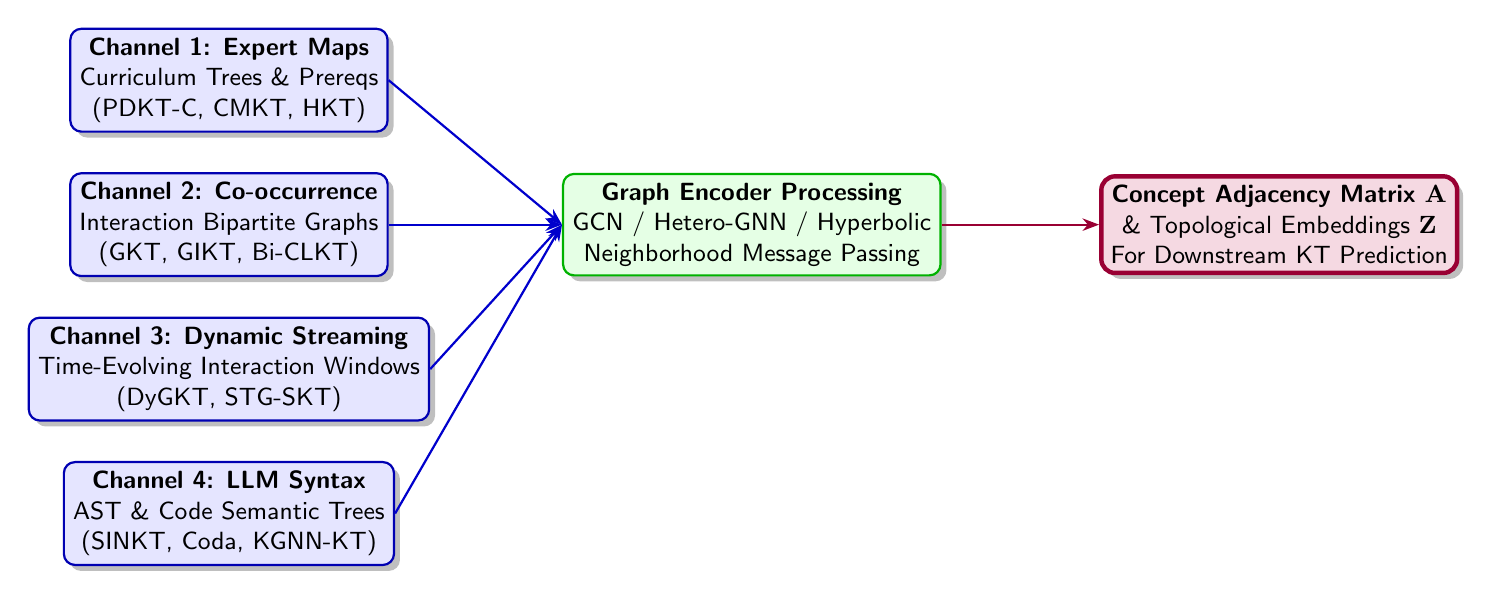
\begin{tikzpicture}[
    node distance=1.0cm and 1.2cm,
    font=\sffamily\small,
    channel/.style={rectangle, draw=blue!70!black, fill=blue!10, thick, rounded corners=4pt, align=center, minimum width=3.8cm, minimum height=1.1cm, drop shadow},
    process/.style={rectangle, draw=green!70!black, fill=green!10, thick, rounded corners=4pt, align=center, minimum width=3.8cm, minimum height=1.1cm, drop shadow},
    output/.style={rectangle, draw=purple!80!black, fill=purple!15, ultra thick, rounded corners=5pt, align=center, minimum width=4.5cm, minimum height=1.2cm, drop shadow},
    arrow/.style={-{Stealth[length=6pt]}, thick, draw=gray!80}
]

% Channels
\node[channel] (c1) {\textbf{Channel 1: Expert Maps}\\Curriculum Trees \& Prereqs\\(PDKT-C, CMKT, HKT)};
\node[channel, below=0.5cm of c1] (c2) {\textbf{Channel 2: Co-occurrence}\\Interaction Bipartite Graphs\\(GKT, GIKT, Bi-CLKT)};
\node[channel, below=0.5cm of c2] (c3) {\textbf{Channel 3: Dynamic Streaming}\\Time-Evolving Interaction Windows\\(DyGKT, STG-SKT)};
\node[channel, below=0.5cm of c3] (c4) {\textbf{Channel 4: LLM Syntax}\\AST \& Code Semantic Trees\\(SINKT, Coda, KGNN-KT)};

% Processing GNN Encoders
\node[process, right=2.2cm of c2] (gnn) {\textbf{Graph Encoder Processing}\\GCN / Hetero-GNN / Hyperbolic\\Neighborhood Message Passing};

% Graph Representation Output
\node[output, right=2.0cm of gnn] (out) {\textbf{Concept Adjacency Matrix $\mathbf{A}$}\\ \& Topological Embeddings $\mathbf{Z}$\\For Downstream KT Prediction};

% Arrows
\draw[arrow, blue!80!black] (c1.east) -- (gnn.west);
\draw[arrow, blue!80!black] (c2.east) -- (gnn.west);
\draw[arrow, blue!80!black] (c3.east) -- (gnn.west);
\draw[arrow, blue!80!black] (c4.east) -- (gnn.west);

\draw[arrow, purple!80!black] (gnn.east) -- (out.west);

\end{tikzpicture}
\end{document}
